\chapter{Theoretische Grundlagen}\label{ref:basics}
Das Projekt basiert auf einigen theoretische Grundlagen. Dazu zählen
neben Prinzipien und Lerntheorien einige technische Begriffe, deren
Erläuterungen Inhalt dieses Kapitels sind. Dabei handelt es sich großenteils um
eine Kurzfassung der Beschreibungen aus \cite{gruben:2012}.

\section{Prinzipien und Theorien}
\subsection{Lernen}
Das Lernen selbst wird heute als ein Prozess verstanden. Dabei wirken "`mehrere
zentrale psychologische Phänomene (Motivation, Emotion,
Kognition)"'\cite{niegemann:2004} zusammen.

Der Lernprozess besteht dabei aus drei Abschnitten:
\begin{enumerate}
  \item Zunächst werden Eindrücke wahrgenommen. Dabei tragen neue oder
  vergessene Eindrücke zur Umstrukturierung im Gehirn bei.
  \item Umstrukturieren bedeutet, dass Synapsen bewegt und andere Gehirnzellen
  angekoppelt werden.
  \item Mit Wiederholungen wird Wissen persistiert. Es entstehen stabile
  Strukturen, welche einfach und schnell abrufbar sind.
\end{enumerate}
In Abbildung \ref{pic:structSyn} wird diese Umstrukturierung illustriert
\cite{spitzer:2012}.

Von ein LMS wird erwartet, dass es diesen Lernprozess unterstützt. Anfänger
sollen die Möglichkeit erhalten zunächst klein anzufangen und die Grundlagen
eines bestimmten Sachverhaltes kennenzulernen. Fortschreitend können die
Anforderungen und Herausforderungen gesteigert werden, um den Lernprozess zu
unterstützten und zugleich die Motivation aufrecht zu erhalten.

\begin{figure}[H]
\centering
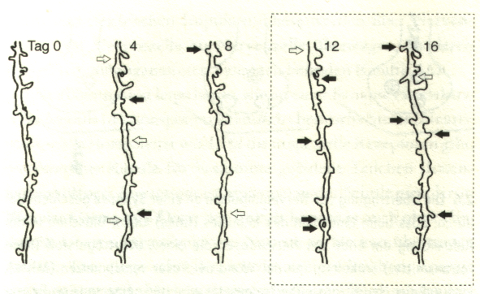
\includegraphics[width=0.7\textwidth]{SPIsynapseS50.png}
\caption{Umstrukturierung von Synapsen \footnotemark}\label{pic:structSyn}
\end{figure}\footnotetext{aus \cite{spitzer:2012}}

\subsection{Motivation}\label{ref:basMotivation}
Die Motivation ist ein wesentliches Standbein des Lernprozesses. Fehlt sie, so
ist es für Lernende bedeutend erschwert, Lerninhalte aufzunehmen, zu verarbeiten
und zu verstehen. Mithilfe von Motivation wird ein charakteristisches Verhalten
an den Tag gelegt, welches den Lernprozess aufrecht erhält \cite{jacobs:2010}.

Im Mittelpunkt jeder Motivation steht stets das persönliche Glück
\cite{stampfl:2012}. Dabei stehen Mittel zur Verfügung, die dem Lernenden auf
unterschliedliche weise unterstützen zu verstehen. Er kann zum einen
intrinsisch und zum anderen extrinsisch motiviert werden.

\subsubsection{Intrinsische Motivation}\label{ref:intrinsischeMotivation}
Die intrinsische Motivation wird auch als direkte Motivation bezeichnet. Damit
wird der Lernende direkt angesprochen und in seinen Bedürfnissen befriedigt und
seinen Wünschen wird unmittelbar nachgegangen. Ein intrinsisch motivierter
Lernender geht einer Tätigkeit im eigenen Interesse nach, es sind keine externen
Einflüsse nötig, die ihn zu seinen Handlungen erst bewegen müssen
\cite{jacobs:2010}.

Jede Lernsoftware hat aus dem zuvor erwähnten Sachverhalt die intrinsiche
Motivation zum Ziel. Dazu werden nicht selten unter Anderem auch gamifizierende
Inhalte verwendet (siehe \ref{ref:gamification}).

\subsubsection{Extrinsische Motivation}\label{ref:extrinsischeMotivation}
Die andere Seite der Motivation kommt von aussen. Es werden Belohnungen gegeben
oder Strafe und negative Konsequenzen vermieden. Synonyme sind demnach
"`indirekte Motivation"', das "`Butterbrot-und-Peitsche-Prinzip"' oder
"`Manipulation"' \cite{jacobs:2010}.

Für Masterly Mate im Speziellen, kann der Tutor ein extrinsisch Motivierender
Faktor sein. Hinzu kommen die gamifizierenden Elemente der zu erreichenden
Punktzahl pro WBT und das Aufsteigen in Rängen. Implizit wird auch Strafe in der
Form angewandt, dass es laut Konzept auch möglich ist, im Rang zu fallen
(siehe dazu Tabelle \ref{tab:privilegesRoles}).

\subsection{Lernmodelle}
Zum Zweck der Unterstützung des Lernprozesses und Förderung der Motivation haben
sich einige Lernmodelle herauskristallisiert, die heute als gültig und
vertretbar angesehen werden. In der Idee von Masterly Mate sind explizit zwei
Lernmodelle verwoben. Das Dreyfus fünf Etappen Modell mentaler Aktivitäten und
Blended Learning.

\subsubsection{Das Dreyfus fünf Etappen Modell mentaler
Aktivitäten}\label{ref:dreyfus}
Inhalt des Dreyfus-Modells ist das Hinterfragen, welche Person einer anderen
einen bestimmten Sachverhalt erklären sollte. Dabei wird insbesondere
berücksichtigt, wie groß der Unterschied der Fachkompetenz zwischen Lernenden
und Lehrenden ist. Es wurden insgesamt fünf Ränge\footnote{Novice, Competence,
Proficiency, Expertise, Mastery} definiert, die den Lernweg von abstrakten
Prinzipien hin zu konkreter Erfahrung mit der Aneignung von Wissen beschreiben
\cite{dreyfus:1980}.

Allgemein formuliert sollte kein Experte einem Neuling etwas erklären. Steigt
man neu in ein Fachgebiet ein, so sind zunächst simple und einfache Beispiele
verbunden mit einem engen Betrachtungswinkel des Sachverhalts sehr hilfreich.
Ein Experte würde den Neuling mit unnötigen Details überhäufen.

Dazu staffelt sich der Lernerfolg in fünf Etappen:
\begin{description}
  \item[1. Novize] Ein Novize ist auf grundlegende Anweisungen angewiesen. Er
  verfügt über kein Vorwissen und evaluiert sich nicht selbst. Mit extrinsischem
  Feedback wird dem Abkommen vom Regelwerk zuvorgekommen.
  \item[2. Fortgeschrittener] Die Handlungen des Fortgeschrittene sind gegenüber
  dem Novizen weniger kontextfrei. Sein weiterer Lernweg kann auf seiner kleinen
  Wissensbasis aufbauen. Er hat grundlegende Prinzipien verstanden und erkennt
  situationsbasierte Muster. Der Fortgeschrittene kann simple Beispiele anhand
  von Guidelines durchlaufen, er experimentiert jedoch nicht.
  \item[3. Erfahrener] Der Umgang mit typischen Situationen am ihm gegebenen
  System stellen keine Hürden für den Erfahrenen dar. Ihm ist es möglich neue
  Situationen anzuknüpfen, einzuordnen und sehr ähnliche bewusst zu
  unterscheiden. Der Erfahrene arbeitet nach selbst erschaffenen Maximen.
  \item[4. Experte] Der Experte ist kein geeigneter Lehrer für einen Novizen
  mehr. Er hat die grundlegenden Prinzipien verloren und arbeitet nach seiner
  Intuition, einer Mischung aus Regeln, Guidelines und Maximen. Lösungen für
  ungewohnte Situationen gehören stets zum Reportoir des Experten. Im Sinne der
  fachlichen Kompetenz ist dieser Grad der höchste.
  \item[5. Meister] Ein Meister zeichnet sich gegenüber dem Experten neben
  fachlicher Kompetenz durch herausragende didaktische Fähigkeiten aus. Er
  bleibt damit auch ein geeigneter Lehrer für Novizen.
\end{description}

Generell sollte sich ein Lehrer zwei Grade über seinem Schüler befinden oder
Meister sein. Weitere detailliertere Erklärungen zu den Rängen finden sich in
\cite{gruben:2012}.

\subsubsection{Blended Learning}\label{ref:blendedLearning}
Zweck des Blended Learning, zu deutsch auch Integriertes Lernen genannt, ist das
Verschmelzen der Vorteile diverser Lernformen. Darunter befinden sich
\ac{F2F}-Education, \ac{DE} und \ac{OE} (eLearning). Die jeweiligen Nachteile
wurden dabei weitestgehend überwunden \cite{kroeger:2004}.

Masterly Mate verfolgt die Verschmelzung von F2F-Education, der Durchführung von
Präsenzunterricht, mit eLearing, dem Durcharbeiten von WBTs. Die DE wird dabei
nur am Rande betrachtet, da nur in Ausnahmefällen Unterweisungen über Chats oder
ähnliche Kommunikationskanäle vonstatten gehen sollen.

\subsection{eLearning}\label{ref:basELearning}
Mit dem eLearning wird im Gegensatz zum regulären Lernprozess ein zusätzlicher
Mittler, eine elektronische Komponente, zwischen die rohen Informationen und dem
lernenden Individuum eingeschoben. Heute ist beispielsweise ein Webbrowser ein
Wiedergabemedium von Vielen, welches der Demonstration von Informationen dient
\cite{baumgartner:2002}.

\subsubsection{Vorteile}
ELearing ist grundsätzlich unabhänig von physischen Gegebenheiten, mithilfe von
Software lassen sich sämtliche, auch fiktive, Szenarien darstellen. Der
Kreativität sind keine Grenzen gesetzt. Auch ist eine enorm vereinfachte
Auswertung von Prüfungen und Tests möglich, da Computer zur Automatisierung von
Prozessen geschaffen sind. 

Für Masterly Mate bedeutet das, dass das Aufsteigen in höhere Ränge
automatisiert vonstatten gehen kann. Beim Überschreiten bestimmter Schwellwerte für Punkte
steigt der Lernende wie von selbst einen Rang auf. Es wird zudem möglich,
Statistiken für den Nutzer anzufertigen, was das Prinzip des gamifizierens
(siehe Abschnitt \ref{ref:gamification}) zusätzlich unterstützt. Das
Masterly Mate selbst ein digitales Produkt ist, spielt darüber hinaus der
eigenen vereinfachten Verbreitung über nationale Grenzen hinweg stark zu.

\subsubsection{Nachteile}  
Grundsätzlich ist der Unterschied zwischen Mensch und Maschine der größte
Gegner von eLearning. Ein Computer kann heute nur recht spärlich auf die
Bedürfnisse des Lernenden eingehen. 

Expertensystemen wird beispielsweise nur eine beratende Funktion zugeteilt.
Weitere Beispiele sind neuronale Netze, welche zwar Lösungen entwickeln können,
jedoch muss deren Erarbeitung überwacht und hinterfragt werden
\cite{keller:2000}.

Letztlich kann das Lernen am Computer heute nicht die Qualität bieten, die ein
Lernender mit einer Lehrkraft erfährt. Seit 1989 entstehen die selben
Diskussionen um den Einsatz von eLearning in Schulen \cite{thome:1989}.

Im Konzept für Masterly Mate werden diese Nachteile berücksichtigt. Wie in
Abschnitt \ref{ref:blendedLearning} beschrieben, baut der Ansatz nicht allein
auf eLearning. Die Nachteile sind erkannt und werden soweit möglich durch die
Verbindung mit Präsenzveranstaltungen gemildert.

\subsection{Flow}\label{ref:basFlow}
Der Flow ist ein Gefühl des völligen Aufgehens in einer Tätigkeit, bei der
die Handlungsschritte als einheitliches Fließen von einem Augenblick zum
nächsten erlebt wird. Einem alltäglichen enthropischen
Zustand\footnote{ungeordnet und zufällig} des Bewusstsein steht im Flow ein
negentrischer Zustand gegenüber. Daher lässt sich annehmen, dass eine Person im
Flow sich auf ihrem höchsten Leistungsniveau befindet
\cite{csikszentmihalyi:1993}.
 
\subsubsection{Komponenten}
Nach diversen Befragungen und Untersuchungen ergaben
sich vier Komponenten, die einen Flow charakterisieren
\cite{csikszentmihalyi:1993}.
\begin{description}
\item[Verschmelzen von Handlung und Bewusstsein] führt dazu, dass sich die
Person als Teil der Handlung sieht. So fühlt sich beispielsweise ein Kletterer
als Teil des Felsens an dem er klettert.
\item[Zentrierung der Aufmerksamkeit auf einen beschränkten Umweltausschnitt]
sorgt dafür, dass von der Handlung unabhängige Reize kaum ins Bewusstsein
gelangen. Die Konzentration liegt im Wesentlichen auf der Gegenwart, währen die
Zukunft und Vergangenheit verschwimmt.
\item[Selbstvergessenheit] ist die Eigenschaft, die die Person im Flow sich
selbst als wahrgenommene Steuerungsinstanz weitestgehend vergessen lässt. Dabei
rücken Selbstzweifel und Sorgen, sowie selbstwertsteigernde Kognitionen in den
Hintergrund.
\item[Ausüben von Kontrolle über Handlung und Umwelt] lässt die Person die
Handlung als kontrolliert wahrnehmen.
\end{description}

\subsubsection{Bedingungen}
Flow ensteht nicht von allein. In der Forschung wurden zwei wichtige Bedingungen
gefunden, die einen Flow begünstigen \cite{csikszentmihalyi:1993}.
\begin{description}
\item[Passung von Fähigkeit und Anforderungen] erfordert ein Gleichgewicht von
Leistungsfähigkeit des Handelnden und die Anforderungen der Tätigkeit. Es ist
stets eine Gradwanderung zwischen Langeweile und Angst aus subjektiver Sicht
des Handelnden. Trifft niedrige Anforderung auf niedrige Fähigkeit, so führt
dies zu Apathie als Gegenspieler von Flow.
\item[Eindeutigkeit der Handlungsstruktur] definiert ein klares Ziel für die
handelnde Person. Dazu gehört, dass keine langwierigen Überlegungen über die
Anforderungen oder mögliche Teilziele notwendig sind. Eine eindeutige Struktur
führt klare Handlungsanforderungen und -möglichkeiten auf und sorgt für
eindeutige und widerspruchsfreie Rückmeldungen. 
\end{description}


\subsection{Gamification}\label{ref:gamification}
Ganz nach dem Claim "`Fun is just another word for learning"'\cite{koster:2005},
werden heute mithilfe von Gamification ernste Inhalte mit spielerischen
Elementen versehen. Damit sollen diese dank geförderter intrinsischer
Motivation (siehe Abschnitt \ref{ref:intrinsischeMotivation}) einfacher zu
vermitteln sein. Als ein modernes Buzzword zu diesem Themengebiet sind heute
"`Serious Games"'\footnote{mitunter populäre Spiele, wie Assassins Creed, in
denen Lerninhalte im Spielkontext verwoben sind \cite{breitlauch:2013}} zu
nennen.

In Bezug auf eLearning ist die Aufgabe des Gamification den Nutzer an die
Anwendung zu binden. Möglich wird dies durch das okkupieren von Aufmerksamkeit
und Bestrebungen mithilfe positiver Eindrücke oder Belohnungen. Als konkrete
Mittel zählen:
\begin{itemize}
  \item Ziele, die den Flow (siehe Abschnitt \ref{ref:basFlow}) des
Nutzers unterstützen,
	\item regelmäßiges Feedback,
	\item eine Messung des Fortschritts,
	\item Belohnung des Aufwandes und der Planerfüllung, nicht nur des Erfolgs und
	\item Motivation von gleichgestellten Nutzern
\end{itemize}
Darüber hinaus kann ein Alleinstellungsmerkmal konzipiert und eine ansprechende
Darstellung entworfen werden. So wird die Anwendung als exotisch angesehen, was
bei einer stimmigen Menge an besonderen Eigenschaften die Motivation zur Nutzung
fördert \cite{raymer:2011}. Im Gegenzug ist es eher Nachteilig, wenn die
Anwendung überladen oder aufdringlich wirkt. Es muss also ein gesundes Mittel
gefunden werden.

Masterly Mate macht sich die motivierende Wirkung von Gamification zunutze. Es
werden Fortschrittsbalken und Statistiken integriert. Zusätzlich erhält er mit
höheren fachlichen Level mehr Möglichkeiten zur Gestaltung seines Profils oder
als Tutor für Gleichgesinnte. Wie die Idee des Gamification in Masterly Mate
konkret konzeptioniert wird, ist Inhalt von Abschnitt
\ref{ref:gamificationConcept}.

\subsection{freie Lizenzen}\label{ref:freeLicenses}
Das reguläre Urheberrecht bietet Autoren wenig Freiheit in Bezug auf die
Freigabe ihrer Werke. Daher entstand aus der Idee der freien Software das
Kreieren einer Lizenz, die dies ermöglicht.

Drei Faktoren zeichnen eine freie Lizenz aus. Autoren erhalten "`ein leicht
handhabbares und frei verfügbares Instrument"'\cite{kreutzer:2011}. Damit können
sie ihre Werke mehr oder weniger frei verbreiten. Nutzer erhalten "`sehr weit
gehende Freiheiten der hierunter stehenden Werke"'\cite{kreutzer:2011}. Darüber
hinaus "`sind die Rechte und Pflichten, die durch die Open-Content-Lizenzen
aufgestellt werden, im Normalfall transparent und leicht zu
verstehen"'\cite{kreutzer:2011}. 

Demnach fasst eine freie Lizenz analog zum Urheberrecht Spielregeln im Umgang
mit urheberrechtlich geschütztem Material dar. Der Unterschied bei der freien
Lizenz liegt dennoch in einer einfacheren Handhabbarkeit und der Übergabe von
Rechten an Nutzer.

Das Projekt zur vorliegenden Studienarbeit bedient sich den Eigenschaften einer
freien Lizenz, um es weiter wachsen zu lassen. Mit der freien Verbreitung soll
sich das Konzept und die Qualität von Masterly Mate mit der Beteiligung
interessierter Personen weiter fortentwickeln.

\section{Konzepte und Implementierungen}
\subsection{Learning Management System}
Ein LMS unterstützt das selbstgesteuerte Lernen. Ein Nutzer arbeitet sich,
möglichst intrinsisch motiviert, durch die ihm dort gebotenen Inhalte
\cite{wendt:2003}.

Wie in der Einleitung beschrieben ist Masterly Mate selbst ein LMS. Der Lernende
entscheidet sich selbst für ein Themengebiet (Topic), welches ihn interessiert.
Dazu findet er WBTs, die ihm bestimmte Sachverhalte auf seinem fachlichen Niveau
näher bringen. Masterly Mate geht mit der Vermittlung von Tutoren über die
eigentliche Definition des LMS hinaus, was es von existierenden OpenSource-LMS,
wie Moodle abgrenzt.

\subsection{Autorenwerkzeug}
Masterly Mate erfordert das Einbinden von WBTs. Autorenwerkzeuge als
\ac{WYSIWYG}-Editoren dienen deren Erstellung und machen laut Definition das
Einbringen von Multimedia möglich \cite{niegemann:2004}. 

In vielen LMS sind heute simple Autorenwerkzeuge integriert. Externe Lösungen
hingegen lassen sich je nach ihren Möglichkeiten und der Handhabung in
professionelle Autorensysteme, WYSIWYG-Editoren und Rapid Content Development
klassifizieren \cite{niegemann:2004}. Masterly Mate unterstützt mit der
Einbindung von SCORM (siehe Abschnitt \ref{ref:scorm}) alle Varianten und bietet
demgegenüber kein eigenes Werkzeug zum Erstellen von Inhalten an.

\subsection{WBT}\label{ref:basWBT}
Beim Begriff des WBTs handelt es sich um eine Softare, die Web-Technologien
nutzt, um eLearning zu realisieren. Blickt man tiefer in die Definition, so
gehen die Meinungen heute auseinander. Eine Variante ist eine Erklärung von
Peter Baumgartner: "`WBT umfasst die internetgestützte Form des Fernlernens mit
und ohne Betreuung durch Tutoren"'\cite{baumgartner:2002}. Dem hinzuzufügen ist,
dass Web-Applikationen im Allgemeinen auch ohne eine Anbindung an das Internet,
beispielsweise lokal oder in einem kleinen Firmennetzwerk, brauchbar sind. 

In einer weiteren Definition taucht das WBT in einer Klassifikation zwischen
virtuellem Klassenzimmer und \ac{CBT} auf. Es kann damit auf eine tutorielle
Betreuung verzichten und ist stark an die Verfügbarkeit in einem
Computernetzwerk gebunden \cite{schleifer:2003}.

Historisch ist WBT aus \ac{DE}, "`Computer-conveyed education"' und diversen
Internet Technologien entstanden, deren Technologien, Traditionen und Techniken
den Grundstein bilden. Daraus wurden bei der Konzeption von WBT die Vorteile
extrahiert und die Nachteile versucht zu vermeiden \cite{horton:2000}.

\subsection{SCORM}\label{ref:scorm}
\ac{SCORM} ist eine Entwicklung der \ac{ADL}-Initiative. Es soll möglich sein,
auf einfache Art und Weise Trainingseinheiten in LMS einzubinden. Zweck von
SCORM und der damit in Verbindung stehenden \ac{API} ist demach das Schaffen einer
Ebene zwischen einem WBT und einem LMS.

\subsubsection{Aufbau}
Dazu ist SCORM zunächst als ein Paket zu verstehen. Für gewöhnlich erfolgt die
Einbindung in das LMS durch einen Import als ZIP-Datei, welche als Container
fungiert. In Abbildung \ref{pic:scormComponents} ist die Hierarchie von
Verschachtelungen von links nach rechts dargestellt.
\begin{figure}[ht]
\centering
\includegraphics[width=0.7\textwidth]{SCORM-Components}
\caption{Komponenten eines
SCORM-Paketes\footnotemark}\label{pic:scormComponents}
\end{figure}\footnotetext{aus \cite{adl:2011}}

\paragraph{Asset}
Assets sind elektronische Ressourcen für die Verwendung in SCOs. Beispiele sind
Medien, Texte, Bilder, Klänge und Töne, \ac{HTML}-Seiten, Assessment Objekte und
andere elementare Teile. Sie kommunizieren nicht direkt mit dem LMS und werden
in einem SCO nur verlinkt, nicht direkt eingebunden. Assets befinden sich quasi
in einem Lager, in dem Ressourcen für den Einsatz in einem SCO bereit liegen.
Aufgrund der Verlinkungen hat das Editieren eines Assets Auswirkung auf
sämtliche Stellen, an denen es eingesetzt ist \cite{adl:2011}.

\paragraph{SCO}
Ein \ac{SCO} ist die kleinste logische Einheit von SCORM. Aus Sicht
der Designer von Lerneinheiten beinhalten SCOs das eigentliche
lehrreiche Material. Programmierer würden sie eher als
Web-Applikation sehen, welche über Schnittstellen für die
Kommunikation mit einem LMS verfügt \cite{adl:2011}.

\paragraph{Aggregation}
Eine Aggregation oder ein Cluster ist ein Verbund von zusammengehörigen
Aktivitäten. Sie kann SCOs oder andere Aggregationen enthalten. Eine Aggregation
ist keine physische Datei, vielmehr ist sie eine Struktur mit der die Planung
einer Reihenfolge zur Abarbeitung von SCOs und Aggregationen möglich wird. In
der SCORM Manifest Datei kann eine Aggregation zusammengesetzt werden
\cite{adl:2011}.

\paragraph{Organization}
Jede SCORM-Datei enthällt eine Organisation. Diese hat gegenüber Aggregationen
keine inhaltlichen Unterschiede. Organisationen zeichnen sich dadurch aus, dass
sie die Wurzel eines jeden SCORM-Paketes bilden, sie enthalten sämtliche Regeln
zur Abarbeitung des WBTs. Daher werden sie auch Root-Aggregation genannt.
\cite{adl:2011}

\paragraph{Curriculum}
Curricula gehen über die Definition von SCORM hinaus und gehören demnach nicht
mehr zum Standard. Sie werden eher von einem LMS zusammengestellt und überwacht
\cite{adl:2011}. Ohne SCORM wäre die Zusammenstellung Curricula jedoch stark
erschwert, es mangelte an einer Schnittstelle, welche die Kommunikation zwischen
WBT und LMS bereitstellt und damit einer Komponente zur Auswertung der
Etappen.

\subsubsection{Manifest-Datei}
Jedes SCORM-Paket ist laut Standard dazu angehalten eine Manifest-Datei mit dem
namen \textit{imsmanifest.xml} zu enthalten. Darin sind wesentliche
Informationen der Lerninhalte für das LMS enthalten. Es kommuniziert welche
Inhalte wann, wie eingebunden werden sollen. Das Schema der SCORM-Manifest-Datei
ist in Abbildung \ref{pic:scormManifest} abgebildet.

Die Metadaten am Kopf der Datei enthalten zusätzliche Informationen zum WBT, die
nach dem \ac{CAM} aufgebaut sind. Da die Unterschiede zwischen
SCORM-Versionen sehr groß ausfallen, wird im Header neben dem
eigentlichen Schema\footnote{meistens "`ADL SCORM"'} weiterhin die Version
mit angegeben\footnote{zum Beispiel "`2004 4th Edition"'}, um Kompatibilität zu
gewährleisten. 

\begin{wrapfigure}{r}{0.5\textwidth}
%\vspace{-15pt} 
\includegraphics[width=0.5\textwidth]{SCORM-Manifest}
\vspace{-30pt}
\caption{Schema der SCORM-Manifest Datei\footnotemark}\label{pic:scormManifest}
\vspace{-20pt} 
\end{wrapfigure}\footnotetext{aus \cite{adl:2011}}
Darunter finden sich die im vorigen Abschnitt erläuterten Komponenten eines
SCORM-Paktes wieder. Unter dem Tag \textit{organizations} wird die
Root-Aggregation mit ihren Regelungen und der Reihenfolge der SCOs aufgeführt. Ein
Item steht dabei jeweils für ein SCO. Ursprünglich war die Unterstützung
mehrerer Organisationen geplant, heute wird jedoch nur eine einzige unterstützt.

Unter \textit{resources} werden sämtliche Assets aufgezählt, die ein SCO oder
Asset benötigt. Eine Ressource ist als eine Gruppierung von Assets zu
verstehen. So werden nur die Assets geladen, die für das aktuelle Modul
benötigt werden. Der Identifier kann in einer Organization oder in einer anderen
Ressource als Abhängigkeit aufgenommen werden.

\subsubsection{SCORM-API}
Die SCORM-API ist notwendig, um die Kommunikation zwischen LMS und WBT zu
vereinheitlichen. So können WBTs eingebunden werden, die aus dem Autorenwerkzeug
als SCORM-Datei exportiert wurden. Abbildung \ref{pic:scormApi} zeigt, wie die
SCORM-API zwischen dem LMS und dem WBT steht. Der Client verfügt über einen
Web-Browser zum betrachten und Durcharbeiten des WBTs, der in einer Aggregation
angeordneten SCOs. Das LMS stellt als Server die WBTs bereit. Es verfügt über
Nutzerinformationen und Informationen über Lerninhalte. Daneben bietet es dem
Lernenden einen Weg für das Erlangen von Wissen in einem Fachgebiet -- ein
Curriculum -- an.

Technisch realisiert ist die SCORM-API mit JavaScript, einer populären
Programmiersprache für Webanwendungen auf Clientseite. Sie besteht aus
zwei Teilen, einen auf der Client- und einen auf der Serverseite.

\begin{figure}[H]
\centering
\includegraphics{SCORM-API}
\caption{SCORM-API Anbindung\footnotemark}\label{pic:scormApi}
\end{figure}\footnotetext{aus \cite{adl:2011}}

\paragraph{API-Wrapper}
Der Client bindet für jedes SCO einen API-Wrapper ein, der die Zugehörigkeit zu
einem SCORM-Paket sichert. Dieser enthällt darüber hinaus alle Funktionen, die
für die Kommunikation der Inhalte mit dem LMS erforderlich sind.
Ein SCO muss dabei mindestens zwei Aufrufe tätigen. Die Funktion
\textit{doInitialize()} initiiert die Verbindung zwischen dem LMS und dem SCO,
\textit{doTerminate()} hingegen trennt die Verbindung noch vor dem Schließen
eines SCO.

\paragraph{SCORM-RTE}
Im Verantwortungsgebiet für das \ac{RTE} von SCORM liegt das Starten von
Inhaltsobjekten, das Herstellen einer Kommunikation zwischen LMS und SCO und das
Verwalten von Informationen über den Lernfortschritt eines Anwenders. Das RTE
definiert ein Modell, welches seine Arbeit aufnimmt wenn ein spezifisches
Inhaltsobjekt zum starten identifiziert wird \cite{adl:2009}.

\subsection{Gestaltungskonzepte}
Da die Arbeit mit Maschinen nicht dem natürlichen Verhalten von Menschen entspricht, 
ist es notwendig Oberflächen von Software zu gestalten, welche von Menschen verstanden und benutzt werden können. 
Es ist dabei besonders wichtig die Menschen, welche mit der Software arbeiten
nicht mit zu vielen Informationen oder 4kompliziertem Verhalten zu überfordern und somit zu frustrieren.
Daher haben sich im Laufe der Zeit einige Gestaltungskonzepte herausgebildet auf die im Folgenden eingegangen werden soll. 

\subsubsection{Die Sinne des Menschen}

Der Mensch verfügt über ein breite Spektrum an Sinnesorganen. Mit diesen kann er 
sich in seiner Umwelt zurechtfinden um mit ihr interagieren zu können. Im Bezug auf die 
Arbeit mit Software wird jedoch meist nur ein Teil der zur Verfügung stehenden Sinne genutzt. 
Zu diesen zählt neben dem Hören vor allem das Sehen, da heutzutage die Kommunikation 
der Maschine zum Menschnen über einen Bildschirm realisiert wird. 

Wie bereits erwähnt erhält der Mensch die Informationen, welche eine Maschine ihm 
zur Verfügung stellt meist über seinen Visuellen Sinn. Damit Menschen diese Informationen ohne 
größere Schwierigkeiten verarbeiten können, ist es wichtig die einzelnen Objekte sinnvoll anzuordnen. 
Hierfür gibt es einige Grundsätze.

\subsubsection{Gesetz der Nähe}  

Das Menschliche Gehirn erkennt Gruppen von Objekten bereits ohne ihre eigentlichen Eigenschaften zu kennen. 
Dies liegt daran, dass Objekte welche nahe beieinander liegen vom Gehirn als zusammengehörend identifiziert. 
Es leuchtet daher ein, dass eine falsche Anordnung von Objekten dem Gehirn falsche Zugehörigkeiten vorgaukelt. 
Der Mensch wird daher Objekt die logisch zusammengehören aber falsch positioniert wurden auch an den 
falschen Stellen suchen. Würde man z.B. in einer Benutzeroberfläche, die
Eingabe von Vor- und Nachname an weit voneinander entfernte Positionen
schreiben, so würden die Benutzer eines der beiden Felder erst spät oder
möglicherweise gar nicht finden. Dies würde die Arbeit mit der
Software erschweren und sie zäh und ineffizient machen.

\subsubsection{Gesetz der Gleichheit}

Dieses Gesetz wirkt nicht so stark, wie das Gesetz der Nähe. Dennoch sollte es
nicht außer acht gelassen werden. Das Gehirn gruppiert neben nah benachbarten
Objekten auch gleichförmige und Gleichartige. So erkennt das Gehirn, dass
Objekte gleiche Farbe in einem direkten zusammenhang stehen müssen und wird sie
daher entsprechend logisch verknüpfen. Bei der Farb-/Formgebung ist daher darauf
zu achten. Die Verwendung von Farbe sollte ohnehin nur mit Maß und Ziel
umgesetzt werden. Darauf wird später näher eingegangen werden.

\subsubsection{Software Ergonomie}

Es gibt einige Grundsätze im Bezug auf die Ergonomie von Software. Die folgenden
sind unter anderem Teil der ISO 9241. 

\paragraph{Aufgabenangemessenheit (ISO)}

Es ist wichtig, dass eine Benutzoberfläche so gestaltet ist, dass die Benutzer
ihre Aufgaben effktiv und effizient erledigen können. D.h. die Software muss
ihnen die benötigten Werkzeuge an die Hand geben um die Aufgaben zu erledigen 
und obendrein müssen diese auch so einfach und intuitiv zu bedienen sein, dass
diese Erledigung in einem zeitlich Vertretbaren Rahmen passieren kann. Die
Software muss daher den Benutzer auf sinnvolle Art und weise unterstützen.
Beispielen für einen solche Unterstützung wäre die Verwendung von Standardwerten
in Textfeldern und/oder Drop-Down-Menus. 

\paragraph{Selbstbeschreibungsfähigkeit (ISO)}

Damit ein Benutzer die Software gut verstehen und damit auch gut bedienen kann,
muss die Software in der Lage sein, ihre Funktionsweise selbst zu beschreiben.
Der Benutzer sollte in die Lage versetzt werden, dass er bei jeder ausführbaren
Funktion genau weiß, was diese bewirkt.

\paragraph{Steuerbarkeit (ISO)}

Im Innern fast eines jeden Menschen befindet sich der Wunsch Macht zu haben und
bestenfalls auch auszuüben. Machtlosigkeit hingegen findet der Mensch belastend. 
Daher sollte eine Software einem Benutzer nicht das Gefühl geben, keine
Kontrolle über sie zu haben. Der Benutzer muss in die Lage versetzt werden,
jeden Schritt, den er mit der Software unternimmt wieder Rückgängig machen oder
gar vollständig abbrechen zu können. 

\paragraph{Erwartungskonformität (ISO)}

Der Mensch hängt, so anpassungsfähig er auch sein mag, Gewohnheiten nach. Daher
er sollte eine Software ihn nicht verwirren indem sie altbekannte und weitgehen
allgemeingültige Muster verändert. Dazu zählen z.B. die Menus "Datei" oder
"Bearbeiten". Gut funktionierendes und bekanntes sollte nicht durch
experimentelles ersetzt werden.

\paragraph{Fluchtlinien}

Fluchtlinien sind keine direkt sichbaren Linien, sondern treten implizit durch
die Anordnung von Objekten auf der Benutzeroberfläche auf. Prinzipiell kann man
sagen, dass eine Oberfläche mit sehr vielen Oberflächen "unordentlicher" und
unübersichtlicher wirkt. Daher sollte eine Benutzeroberfläche möglichst wenige
Fluchtlinien aufweisen. Fluchtlinien entstehen durch die Außenkanten von
Objekten. Dies bedeutet, dass eine Anordnug bei denen die Kanten der Objekte auf 
der gleichen Linien liegen, wenige Fluchlinien erzeugen.

\paragraph{Schrift}

Die Schrift sollte angemessen und gut lesbar sein. Bei langen Texten strengt
eineine Serifenlose Schrift das Auge an. Bei Benutzeroberflächen hingegen wirken
diese angemessener. Außerdem ist es wichtig, dass die Schrift gut lesbar ist.

\paragraph{Farben}

Farben sind grundsätzlich sparsam einzusetzen. Außerdem ist beim Einsatz der
Farben zu beachten, dass diese eine Psychologische Wirkung haben. So wird rot in
aller Regel mit Gefahr assoziiert. Man sollte diese Farbe daher auch dafür
einsetzen. Des Weiteren ist zu vermeiden Grundfarben nebeneinander zu verwenden.

\subsubsection{GUI-Bloopers}

Ein Blooper bezeichnet einen Missgriff, in diesem Abschnitt geht es daher um
Missgriffe bei der Gestaltung von Benutzeroberflächen. Einige werden im
folgenden vorgestellt.

\paragraph{Dynmamische Menus}

Menus die im Verlauf der Arbeit mit der Software ihren Inhalt ändern. Dies mag
auf den ersten sehr innovativ wirken, verwirrt den Benutzer aber nur unnötig.

\paragraph{Checkboxes und Radiobuttons falsch einsetzen}

Checkboxen sollten nur verwendet werden, wenn es sich bei der abgebildeten
Funktionalität tatsächlich um eine An-/Auswahl handelt.

\subsection{Autorisierung und Authentifikation}
Die Authentifikation bezeichnet den Anmeldevorgang eines Nutzers an einem
System. Der Grundgedanke bei der Authentifikation ist, dass lediglich
berechtigten Nutzern der Zugang zu vertraulichen Daten gewährt werden soll.
Grundlegend unterscheidet man bei einer Authentifikation zwischen der
Identifizierung und dem Beweis der Identifizierung. Diese beiden Schritte sind
bei einer Authentifikation unumgänglich. Die Identifizierung leitet den ersten
Schritt einer Authentifikation ein. Dabei wird der Nutzer darauf aufgefordert,
seine eindeutige Benutzerkennung anzugeben. In vielen Systemen werden
vorgegebene Standardbenutzerkennungen eingesetzt. Falls einem Angreifer eine
Benutzerkennung bekannt ist, so muss dieser lediglich den zweiten Schritt der
Authentifikation, nämlich dem Beweisen der Identifikation, am System
durchführen, um Zugang zu vertraulichen Daten zu erhalten. In diesem Fall gibt
sich der Angreifer mit einer anderen Identität aus. Man spricht dann auch von
Impersonation. Um eine Impersonation zu vermeiden, ist es ratsam bei produktiven
Systemen, bereits bei der Vergabe von vorgegebenen Benutzerkennungen andere zu
verwenden, die von den häufig verwendeten Standardbenutzerkennungen abweichen.
Eine erheblich schwierigere Hürde für einen Angreifer stellt allerdings der
zweite Schritt der Authentifikation dar - dem Beweisen der Identifikation,
welches auch als Authentifizierung bezeichnet wird.
Man unterscheidet dabei mehrere Authentifizierungsverfahren, die nach den
Aspekten Wissen, Besitz und biometrische Verfahren klassifiziert werden können.

\subsubsection{Wissen}
Ein Benutzer weiß etwas, was andere Benutzer nicht wissen. Die häufigste
Anwendung die unter diese Klassifikation fällt, ist die Verwendung von
Passwörtern.

\subsubsection{Besitz}
Der Benutzer besitzt etwas, das andere Benutzer nicht besitzen. Dies könnte z.B.
ein Schlüssel zu einem Raum oder Gebäude sein.

\subsubsection{Biometrische Verfahren}
Bei diesen Verfahren wird vorausgesetzt, das die zu verifizierenden Objekte
untrennbar vom Benutzer sind. Das könnte z.B. ein Finger sein, der für einen
Fingerabdruck benötigt wird.

Bei der Authentifizierung besitzt der Nutzer viele Möglichkeiten, um den Zugang
für unberechtigte Personen zu erschweren. Bei der Verwendung von Passwörtern
kann durch die Länge und die Anzahl der genutzten Sonderzeichen eine sehr hohe
Komplexität geschaffen werden, bei der der Angreifer eine Vielzahl an
Kombinationen berücksichtigen müsste. Allerdings reicht dies alleine noch nicht
für den Schutz vor Angreifern aus. Das meist in der Datenbasis hinterlegte
Passwort darf in keinem Fall als Klartext persistiert werden. Daher entscheidet
die Wahl eines geeigneten Verschlüsselungsverfahren im
Wesentlichen über die Sicherheit gegen den unberechtigten Zugang. Viele Systeme
nutzen als Verschlüsselung für Passwörter den MD5-Hash. Für eine
wesentlich höhere Sicherheit sorgt heutzutage allerdings ein SHA-Hash.

Die Autorisierung bezeichnet im Wesentlichen die Vergabe von Zugriffsrechten für
Benutzer oder Gruppen auf bestimmte Ressourcen. Damit regelt die Autorisierung
im Gegensatz zur Authentifizierung, welches die Zugangskontrolle festlegt, die
Zugriffskontrolle. Für die Autorisierung können verschiedene Verfahren
eingesetzt werden, um den Zugriff bestimmter Benutzer oder Gruppen auf
entsprechende Ressourcen zu regeln. Die Whitelisting und Blacklisting
Verfahren fallen dabei unter die einfachsten Zugriffsverfahren. Dabei werden
einzelne Benutzer sogenannten Whitelisten hinzugefügt, um kenntlich zu machen,
welche Nutzer auf die entsprechende Ressource zugreifen können. Alle Nutzer, die
nicht in der Liste aufgeführt sind, besitzen demnach keinen Zugriff auf die
Ressource. Im Gegensatz zum Whitelisting werden beim Blacklisting die Nutzer
bzw. Subjekte aufgeführt, die keinen Zugriff auf eine Ressource erhalten. Alle
anderen Nutzer, die sich nicht auf der Liste befinden, erhalten einen Zugriff.
Das Whitelisting-Verfahren wird allerdings meist dem Blacklisting bevorzugt, da
die Anzahl der nichtberechtigten Nutzer auf eine Ressource in den meisten
Szenarien größer ist als die Anzahl berechtigter Nutzer. Bei Anti-Virenscannern
wird aber z.B. eher das Blacklisting für die Filterliste eingesetzt.
Für die Zugriffskontrolle auf Dateisystemen werden heutzutage meist 
Matrixmodell wie z.B. ACL \footnote{Access Control List} verwendet.

\subsection{Ruby on Rails}
\ac{RoR} ist ein in der Programmiersprache Ruby programmiertes Framework für die
einfache Enwicklung von Web-Applikationen. Das Design folgt Annahmen über
grundlegende Voraussetzungen, welche jeder Programmierer zu Beginn benötigt.
Darüber hinaus ist weniger Programmcode zum Erreichen von Zielen
erforderlich \cite{railsGuides:2013}.

\subsubsection{Handhabung}
Das Erstellen einer RoR-Applikation folgt einem recht eigensinnigen Weg. Ein
"`bester"' Weg wird als Annahme vom Framework unterstützt. Alternativen führen
demgegenüber gelegentlich zum Gegenteil und die Implementierung wird erschwert.
Ein Programmierer ist daher angehalten sich den "`Rails Way"' anzunehmen, um
eine beschleunigte Produktivität im Gegensatz zu weniger produktiven
Ergebnissen zu erreichen. Die drei folgenden Prinzipen sind in RoR fest
eingewoben und sollten verinnerlicht werden \cite{railsGuides:2013}:
\begin{description}
\item[DRY] "`Don't Repeat Yourself"' empfielt es, den selben Programmcode nicht
immer wieder erneut zu schreiben. Eine durchdachte Architektur macht Objekte und
Methoden leicht wiederverwendbar.
\item[Convention over Configuration] RoR macht annahmen darüber, wie Ziele
erreicht werden wollen und beugt so das schier endlose Durcharbeiten von
Konfigurationsdateien vor.
\item[REST] mit dem \ac{REST}-Muster (siehe Abschnitt \ref{ref:basREST}), mit
dem eine Web-Applikation aus Ressourcen und standard HTML gefertigt wird, macht diese performanter
\item[MVC] wird in Abschnitt \ref{ref:basMVC} näher erläutert
\end{description}

\subsubsection{Komponenten}\label{ref:baseGem}
RoR selbst ist sehr modular aufgebaut, um die gewünschten Anforderungen
bestmöglich erfüllen zu können. Die einzelnen Komponenten werden "`gems"'
genannt. Jeder Interessierte kann nach belieben eine neue gem schaffen oder eine
vorhandene verbessern. Tabelle \ref{ref:tabRoRComp} zeigt die gems aus denen RoR
selbst besteht \cite{railsGuides:2013}.

\begin{longtable}{|p{1.8cm}|p{12.5cm}|}
\caption{Ruby on Rails Komponenten\footnotemark}\label{ref:tabRoRComp}\\\hline

\endfirsthead

\multicolumn{2}{c}{\tablename\ \thetable{} (Fortsetzung)} \\\hline
\endhead

\hline \multicolumn{2}{|r|}{{Fortsetzung auf der nächsten Seite \ldots}}\\\hline
\endfoot

\hline
\endlastfoot

\textbf{Action Pack}&Dieses gem realisiert das VC in MVC. Es besteht aus Action
Controller, Action Dispatch und Action View.

Der \textbf{Action Controller} verwaltet die Controller in einer Rails
Applikation.
Das zugehörige Framework vermittelt eingehende Anfragen zu einer Rails
Applikation, extrahiert Parameter und sendet sie zur vorgesehenen Action. Die
bereitgestellten Dienste des Action Controllers umfassen das Sitzungsmanagement,
das rendern von Templates und die Verwaltung von Umleitungen.

\textbf{Action View} Demgegenüber ist Action View verantwortlich für die
Verwaltung der Views der Applikation. Es ist standardmäßig in der Lage HTML und
XML\footnotemark zugleich auszugeben. Es rendert Templates und inkludiert
eingebettete Templateteile\footnotemark und die eingebaute
AJAX\footnotemark-Unterstützung.

\textbf{Action Dispatch} verwaltet das Routen von Web-Anfragen und leitet diese
beliebig an die eigene oder eine andere Applikation weiter. \\\hline

\textbf{Active Mailer}& Dieses Framework stellt E-Mail Dienste her.
Eingehende E-Mails können verarbeitet werden oder neue E-Mails können
als einfacher Text oder als mehrteilige Dokumente aus flexiblen
Templates generiert und schließlich gesendet werden.\\\hline

\textbf{Active Model}&Active Model stellt ein definiertes Interface
zwischen den Action Pack Diensten und Mapping von Objektbeziehungen
bereit. Dieses gem erlaubt RoR die Verwendung eines alternativen
ORM\footnotemark-Frameworks, falls dies für die Applikation benötigt
wird.\\\hline

\textbf{Active Record}&Die Basis für Models in RoR ist Active Record. Es bietet
unter Anderem Datenbankunabhängigkeit, grundlegende
CRUD\footnotemark-Funktionalität, erweiterte Suchmöglichkeiten und die Fähigkeit
Relationen zwischen Models herzustellen.
\\\hline

\textbf{Active Resource}&Die Verwaltung der Verbindung zwischen Objekten
und RESTful Webservices stellt Active Resource bereit. Es implementiert
einen Weg webbasierte Ressourcen an lokale Objekte mittels CRUD Semantiken zu
binden.\\\hline

\textbf{Active Support}&Active Support ist eine umfangreiche Sammlung
von Werkzeugklassen und standard Ruby Bibliothekserweiterungen, welche
in RoR Verwendung finden.\\\hline

\textbf{Railties}&Railties ist der Kerncode von RoR, welcher neue
Applikationen baut und die aufgeführten Frameworks und Plugins zu einer
allumfassenden Applikation verbindet.\\\hline

\end{longtable}\footnotetext[24]{aus
(\cite{railsGuides:2013})}\footnotetext[25]{\acl{XML}}\footnotetext[26]{genannt
"`partials"'}\footnotetext[27]{\acl{AJAX}}\footnotetext[28]{\acl{ORM}}\footnotetext[29]{\acl{CRUD}}

\subsection{REST}\label{ref:basREST}
REST ist die Basis für eine von Roy Fiedling entworfene RESTful Architektur
\cite{fiedling:2000}. Demnach besteht REST in Bezug auf RoR im Wesentlichen aus
zwei Prinzipien: Es werden zum einen Identifizierungen für Ressourcen analog
\ac{URI}s verwendet, um Ressourcen zu repräsentieren. Zum anderen werden
Repräsentationen des Status der Ressource zwischen Systemkomponenten
transferiert.

Beispielsweise wird unter dem HTTP Request \textit{DELETE /photos/17}
verstanden, dass zu einer Ressource Photo mit der ID 17 verwiesen werden soll.
Zusätzlich wird eine gewünschte Aktion indiziert, die das Löschen der Ressource
veranlasst. REST ist damit ein recht natürlicher Stil für die Architektur von
Webapplikationen. RoR greift REST auf und versteckt gleichzeitig einige
REST-Komplexitäten und Bowser Eigenarten \cite{railsGuides:2013}.

\subsection{MVC Architektur}\label{ref:basMVC}
\ac{RoR} baut auf der \ac{MVC}-Architektur, dessen Komponenten und Eigenschaften
in Tabelle \ref{ref:tabMVC} zu sehen sind, auf. Damit ist es möglich, die
Programmcodes für Programmlogik und Nutzerinterface sauber zu trennen. So ist es
einfacher Programmteile zuzuordnen, was eine einfachere Wartung garantiert.
Darüber hinaus kann so das \ac{DRY}-Prinzip sehr einfach umgesetzt werden
\cite{railsGuides:2013}.

\begin{table}[ht] \centering \caption{Komponenten der MVC-Architektur und deren
Eigenschaften\footnotemark}\label{ref:tabMVC}
\begin{tabular}{|p{2cm}|p{12cm}|}\hline 
\textbf{Model}&Ein Model repräsentiert
die Informationen (Daten) der Applikation und die Regeln zu deren Manipulation.
In RoR werden Models primär für die Handhabe von Regeln zur Interaktion mit der
korrespondierenden Datenbanktabelle verwendet. Üblicherweise wird ein Model auf
eine Datenbanktabelle abgebildet. Der Großteil der Programmlogik wird in Models
abgebildet.\\\hline 

\textbf{View}&Views repräsentieren das Nutzerinterface der
Applikation und stellen Informationen für den Web-Browser oder andere Werkzeuge
bereit, welche Anfragen an die Applikation stellen. In RoR sind dies meistens
HTML-Dateien mit eingebettetem Ruby-Programmcode, der allein für das Darlegen
von Informationen zuständig ist.\\\hline
 
\textbf{Controller}&Controller sind quasi der Kleber zwischen Model und
View. In RoR nehmen die Controller die Anfragen an den Webserver
entgegen, sie fragen Daten aus der Datenbank bei den Models ab und
übergeben diese an die Views zur Präsentation.\\\hline
\end{tabular}
\end{table}
\footnotetext{aus \cite{railsGuides:2013}}